

%------------------------------------------------
\section{Entregables}
%------------------------------------------------



\begin{frame}
\frametitle{Reporte Técnico de Desarrollo de Práctica}
\begin{itemize}
\item Para cada práctica realizada, entregar un documento (\textbf{únicamente en formato PDF*}) con las siguientes secciones:
\begin{itemize}
\item Introducción
\item Desarrollo Experimental
\item Resultados
\item Conclusiones
\item \textbf{Referencias}
\end{itemize}
\item Para GENERAR este reporte es necesario utilizar la plantilla en LATEX (\textbf{únicamente usando LATEX*}) localizada en el siguiente enlace:
\url{https://www.overleaf.com/read/dgkhvfwnygvc}
\end{itemize}
\end{frame}

\begin{frame}
\frametitle{Reporte Técnico de Desarrollo de Práctica}
\begin{itemize}
\item Bajo ninguna circunstancia deben incluir \textbf{CÓDIGO FUENTE}. Si pueden incluir diagrama de flujo, Pseudocódigo, Diagrama E-R, Diagrama de Clases, de Casos de USO, etc. De incluir código fuente, solo tendrá un 50\% del valor en la calificación. 
\item En caso de trabajos indivudales o en EQUIPO, deben emplear la plantilla LaTex que se provee. En caso de utilizar algo diferente a LaTex u otra plantilla de LaTex, la calificación proporcional del informe será \textbf{DESESTIMADA}. 
\item En caso de trabajos en equipo, se debe agregar los integrantes al inicio del INFORME. \textbf{El trabajo solo cuenta para aquellos integrantes mencionados en el informe (y que dicho nombre se encuentre registrado tal cual en la lista). Una vez ENTREGADO, si hay OMISIONES de los integrantes, no se realizará CORRECCION alguna, se debe asumir la consecuencias que esto conlleva. }
\end{itemize}

\end{frame}


\begin{frame}
\frametitle{Ponderación del Informe en la Calificación del Proyecto}
\begin{itemize}
\item Proyecto: 66 Puntos
\begin{itemize}
\item Ejecución y Funcionalidad: 45 Puntos
\item Modularidad: 13 Puntos
\item Documentación: 8 Puntos
\end{itemize}
\item Informe: 34 Puntos
\begin{itemize}
\item Uso adecuado de Latex: 5 Puntos
\item Organizaci\'on y Redacci\'on: 6 Puntos
\item Referencias en formato adecuado: 8 Puntos
\item Evidencia del trabajo realizado: 8 Puntos
\item Sin faltas de ortografía ni errores de dedo: 7 Puntos
\end{itemize}
\end{itemize}
\end{frame}

\begin{frame}
\frametitle{Flujo de Evaluaci\'on}
\begin{columns}
\begin{column}{0.5\textwidth}
\begin{itemize}
\item Proyecto que no este entregado de acuerdo con las especificaciones, ser\'a regresado (y penalizado)
\item Puede dar tantas vueltas como el estudiante desee
\item Se recomienda LEER con cuidado la secci\'on de entregables en esta diapositiva
\end{itemize}
\end{column}
\begin{column}{0.5\textwidth}
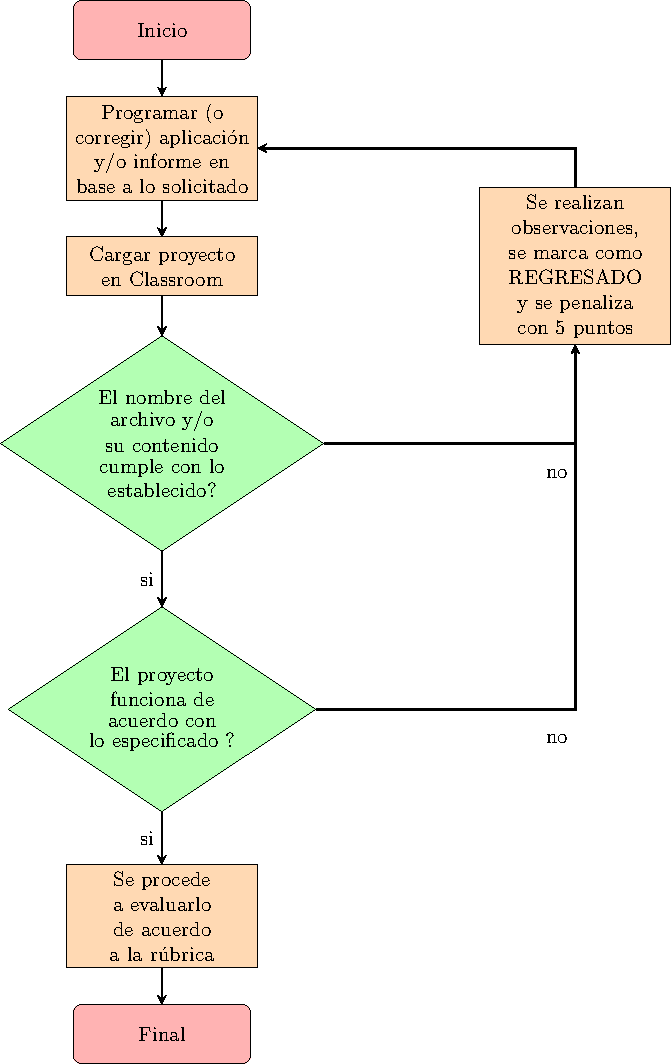
\includegraphics[width=4cm]{DiagramaFlujoVaginal/DF.pdf}
\end{column}
\end{columns}
\end{frame}

%------------------------------------------------


% Actualizacion 
%\begin{frame}
%\frametitle{Entregables de proyecto individual}

%\begin{itemize}
%\item \textbf{Clave de GRUPO (incluir guión medio)}
%\item \textbf{Nombre del integrante iniciando por apellido paterno, SIN ESPACIOS y separado por guion bajo}
%\item \textit{\clavegrupo}\_nuno\_maganda\_marco\_aurelio.zip,  \textit{\clavegrupo}\_nuno\_maganda\_marco\_aurelio.pdf, etc. 
%\end{itemize}
%\textbf{Clave de GRUPO seguido del nombre del integrante iniciando por apellido paterno, SIN ESPACIOS y separado por guion bajo}. 
%\begin{itemize}
%\item A su respectiva carpeta de github, cargar lo siguiente:
%\begin{enumerate}
%\item Archivo .ZIP con el código fuente.
%\item Archivo instalador de la aplicación (.APK).  
%\item Archivo PDF con el informe. 
%\end{enumerate}
%\item Mismo formato de NOMBRE de archivo del ENTREGABLE principal para el nombre de los archivos al interior del ZIP
%\end{itemize}

%\end{frame}


\begin{frame}
\frametitle{Entregables de proyecto individual}
    \begin{itemize}
    \item Crear la carpeta de su repositorio con el siguiente nombre:
    \begin{itemize}
        \item \textbf{\clavegrupo\_uX\_nuno\_maganda\_marco\_aurelio}
    \end{itemize}
    \item La carpeta del repositorio  Github creado para su proyecto individual debe tener lo siguiente:
        \begin{itemize}
        \item \textbf{\clavegrupo\_uX\_nuno\_maganda\_marco\_aurelio\_source} (Carpeta con c\'odigo fuente de la aplicaci\'on)
        \item \textbf{\clavegrupo\_uX\_nuno\_maganda\_marco\_aurelio\_latex} (Carpeta con c\'odigo fuente del informe)
        \item \textbf{\clavegrupo\_uX\_nuno\_maganda\_marco\_aurelio.apk} (Instalable)
        \item \textbf{\clavegrupo\_uX\_nuno\_maganda\_marco\_aurelio.pdf} (Informe)
        \end{itemize}
    \item Donde:
        \begin{itemize}
        \item \textbf{X} es el n\'umero de unidad a un d\'igito (1, 2, etc)
        \item \textbf{Sustituir con sus apellidos y nombres de manera apropiada} 
        \end{itemize}
    \end{itemize}
%\textbf{Cuatro cuatrimestres ignorando estas instrucciones, ya deber\'ia poner nombres y apellidos. El que lo haga ser\'an sentadillas o p\'aginas, ustedes escojan!}
\end{frame}





\begin{frame}
\frametitle{Entregables de proyecto en equipo}
    \begin{itemize}
    \item Crear la carpeta de su repositorio con el siguiente nombre:
    \begin{itemize}
        \item \textbf{\clavegrupo\_eq\_NN\_uX}
    \end{itemize}
    \item La carpeta del repositorio  Github creado para su proyecto en Equipo debe tener lo siguiente:
%\begin{itemize}
%\item \textbf{Clave de GRUPO (incluir guión)}
%\item \textbf{Palabra equipo seguido del numero de equipo (usando dos digitos)}
%\item Por ejemplo: \textbf{\clavegrupo\_equipo\_01.zip} 
%\end{itemize}
%El contenido del archivo debe ser:
\begin{itemize}
\item \textbf{\clavegrupo\_eq\_NN\_uX\_source} (Carpeta con c\'odigo fuente de la aplicaci\'on)
\item \textbf{\clavegrupo\_eq\_NN\_uX\_latex} (Carpeta con c\'odigo fuente del informe)
\item \textbf{\clavegrupo\_eq\_NN\_uX.apk} (Instalable)
\item \textbf{\clavegrupo\_eq\_NN\_uX.pdf} (Informe)
\end{itemize}
Donde:
\begin{itemize}
\item \textbf{NN} es el n\'umero de equipo a dos d\'igitos (01, 02, etc)
\item \textbf{X} es el n\'umero de unidad a un d\'igito (1, 2, etc)
\end{itemize}
\item En cada entrega, \textbf{UN SOLO INTEGRANTE DEL EQUIPO} deberá cargar los siguientes archivos en la carpeta asignada por Github para trabajar
\end{itemize}


%Ejemplos: \textit{claveGrupo}\_equipo\_01.zip, iti-27798\_equipo\_01.pdf, etc
\end{frame}




\begin{frame}
\frametitle{Nombres de Archivos Entregables}
En el caso de nombres y apellidos acentuados, con dieresis o con virgulilla (\textasciitilde{}), sustituir de acuerdo con las siguientes reglas:
\begin{itemize}
\item Sustituir N/n por \~N/\~n
\item Sustituir A/a por \'A/\'a
\item Sustituir E/e por \'E/\'e
\item Sustituir I/i por \'I/\'i
\item Sustituir O/o por \'O/\'o
\item Sustituir U/u por \'U/\'u
\item Sustituir U/u por \"U/\"u
\end{itemize}
\end{frame}



\begin{frame}
\frametitle{Codigo Fuente del Proyecto}
\begin{itemize}
\item Se debe extraer utilizando el SCRIPT para dicho prop\'osito (SOLO EXISTE HAY PARA LINUX, usuarios Windows deben programar el SUYO o replicar los pasos del SCRIPT Linux para sus entrega) que se proveerá en el CLASSROOM para extraer los archivos necesarios
\item \textbf{De ninguna manera se debe compactar la carpeta completa del PROYECTO. De hacer esto, habr\'a una penalizaci\'on de 20 PUNTOS}
\end{itemize}

\end{frame}


\begin{frame}
\frametitle{Nombre de Aplicaci\'on (Al crear su proyecto en Android Studio)}
\begin{itemize}
\item Para los proyectos individuales (en MAYUSCULAS):
\begin{itemize}
\item Nombre de la Aplicacion: Z\_UX\_APAT\_AMAT\_NOMBRE
\item $X$ es Numero de unidad en un digito
\item APAT, AMAT, NOMBRE - Datos del estudiante
\item Z es Z, es para que al instalar la aplicacion quede al final del listado
\end{itemize}
\item Para lo proyectos en equipo (en MAYUSCULAS):
\begin{itemize}
\item Nombre de la Aplicacion: Z\_UX\_CLAVEGRUPO\_E\_NUMEROEQUIPO
\item $X$ = Numero de unidad en un digito
\item CLAVEGRUPO - iti-RRRRRR (RRR los digitos al final de la clave de grupo)
\item NUMERO DE EQUIPO a DOS DIGITOS: 01, 02, 03
\item Z es Z, es para que al instalar la aplicacion  quede al final del listado
\end{itemize}
\end{itemize}

\end{frame}


\begin{frame}
\frametitle{Nombre de Aplicaci\'on (Al crear su proyecto en Android Studio)}
\begin{itemize}
\item Para las aplicaciones en Asignacion Especial (En caso de que se les solicite entregar el APK y el codigo fuente) (EN MAYUSCULAS):
\begin{itemize}
\item Nombre de la Aplicacion: Z\_AEX\_APAT\_AMAT\_NOMBRE
\item $X$ Numero de unidad en un digito (1, 2, 3, etC)
\item APAT, AMAT, NOMBRE = Datos del estudiante
\item Z es Z, es para que al instalar la aplicacion  quede al final del listado
\item Si llegara a ser en equipo, utilizar la nomenclatura de un proyecto en equipo dejando el inicio de la APP sin cambios (Z\_AE$X$)
\end{itemize}
\end{itemize}

\end{frame}

\begin{frame}
\frametitle{Package de su Aplicaci\'on}
\begin{itemize}
\item Para proyectos individuales: \textbf{upvictoria.pm\_ene\_abr\_2024.iti\_271086.pi1u1.nuno\_maganda}
\item Sustituir iti\_271086 por su GRUPO
\item Sustituir nuno\_maganda por sus apellidos paterno y materno respectivamente
\item Ajustar pi1uX para proyectos proyecto invidividuales (proyecto individual 1 unidad X=1,2,3, etc)
\item Si el proyecto es individual, debe llevar los apellidos paterno y materno
\item Para proyectos en equipo: \textbf{upvictoria.pm\_sep\_dic\_2023.iti\_271086.pg1uX\_eqYY}
\item Sustituir iti\_271086 por su GRUPO
\item Ajustar pg1uX para proyectos en equipo (proyecto grupal 1 unidad X = 1,2,3, etc) -
\item donde YY es el numero del equipo a dos digitos
\item Para asignaciones especiales: upvictoria.pm\_sep\_dic\_2023.iti\_271086.ae1uX.nuno\_maganda
\item  donde X es el numero de unidad X (1, 2, etc) 
\end{itemize}

\end{frame}
